\documentclass[compress]{beamer}
\usepackage{irbookslide}
\usepackage{irilmenau2}
\usepackage{tikz}
\usepackage{url}
\usepackage{ifxetex}
%\RequireXeTeX
\usepackage{fontspec} % zahteva paket euenc
\usepackage{xunicode}
\usepackage{xltxtra}
\usepackage{polyglossia}
\usepackage{minted}
\usepackage{algorithmic}
\renewcommand{\algorithmicrequire}{\textbf{Input:}}
\renewcommand{\algorithmicensure}{\textbf{Output:}}
\usepackage{xcolor,colortbl}
\usepackage{textcomp}
%\setdefaultlanguage[script=Latin]{serbian}

\title{Python za Java programere}
\subtitle{izvor: http://python4java.necaiseweb.org}
\institute{Katedra za informatiku, Fakultet tehničkih nauka, Univerzitet u
Novom Sadu}
\date{2019.}
\subject{Predavanja sa OISISI}

\begin{document}

\frame{\titlepage}

\section{Uvod}
\begin{frame}[fragile]
  \frametitle{Python za Java programere}
  \begin{itemize}
    \item izvršavanje programa
    \item osnovne konstrukcije
    \item funkcije i metode
    \item interakcija sa korisnikom
    \item stringovi
    \item grananje i petlje
    \item funkcije
    \item moduli
    \item liste (nizovi)
    \item tekstualni fajlovi
    \item rečnici
    \item klase, veze među klasama
    \item preklapanje operatora
    \item izuzeci
    \item nasleđivanje
    \item kopiranje objekata
  \end{itemize}
\end{frame}

\begin{frame}[fragile]
\frametitle{Izvršavanje Python programa}

Python program je tekstualni fajl koji sadrži naredbe. Primer:

\begin{minted}[linenos=false]{python}
# Classic hello world program in Python.

print("Hello World")
print("How are you today?")
\end{minted}
\end{frame}

\begin{frame}[fragile]
\frametitle{Nema \texttt{main()}}

Prva naredba koja se izvršava je prva naredba u fajlu na globalnom nivou
(izvan svih funkcija i metoda).

U prethodnom primeru, to je prva \texttt{print} naredba.

\begin{minted}[linenos=false]{bash}
python myprogram.py
\end{minted}
\end{frame}

\begin{frame}[fragile]
\frametitle{Shebang za Linux i macOS}

Dodati kao prvi red u fajlu

\begin{minted}[linenos=false]{bash}
#!/usr/bin/python
\end{minted}

Zatim uključiti execute bit:

\begin{minted}[linenos=false]{bash}
chmod +x myprogram.py
\end{minted}

Nadalje se program može pokrenuti i ovako:

\begin{minted}[linenos=false]{bash}
./myprogram.py
\end{minted}  
\end{frame}

\begin{frame}[fragile]
\frametitle{Interaktivni mod}
Poziv Python interpretera:
\begin{minted}[linenos=false,fontsize=\footnotesize]{bash}
$ python
\end{minted}
\begin{minted}[linenos=false,fontsize=\footnotesize]{python}
Python 3.7.4 (default, Jul  9 2019, 18:13:23) 
[Clang 10.0.1 (clang-1001.0.46.4)] on darwin
Type "help", "copyright", "credits" or "license" for more information.
>>> x = 1
>>> y = x + 1
>>> y
2 
\end{minted}
\end{frame}

\section{Osnove}

\begin{frame}[fragile]
\frametitle{Osnovne konstrukcije}
Hello world u Javi:
\begin{minted}[linenos=false,fontsize=\small]{java}
// Hello World in Java.
public class HelloWorld {
  public static void main(String[] args) {
    System.out.println("Hello World");
  }
}
\end{minted}

Hello world u Pajtonu:

\begin{minted}[linenos=false,fontsize=\small]{python}
# Hello World in Python.
print("Hello World")
\end{minted}
\end{frame}

\begin{frame}[fragile]
\frametitle{Format reda}
\begin{itemize}
  \item naredba se ne završava sa tačka-zarez
  \item kraj linije je i kraj naredbe
\end{itemize}
\begin{minted}[linenos=false,fontsize=\small]{python}
print("Hello World!")
print("How are you today?")
\end{minted}

\begin{itemize}
  \item u Javi naredba se završava sa tačka-zarez i može se protezati kroz više
linija:
\end{itemize}
\begin{minted}[linenos=false,fontsize=\small]{java}
// Java statement
System.out.print
  (
    "Hello World!"
    )
;
\end{minted}
\end{frame}

\begin{frame}[fragile]
\frametitle{Format reda}
\begin{itemize}
  \item naredba se može protezati kroz više redova
  \item backslash za nastavak u sledećem redu
\end{itemize}
\begin{minted}[linenos=false,fontsize=\small]{python}
result = (someValue * 5 + anotherValue * 12) \
         - (originalValue * 2)
name = "John "\
       "Smith"
\end{minted}

\begin{itemize}
  \item poziv funkcija ima zagrade, pa se naredba ne mora nastavljati sa 
    backslash
\end{itemize}
\begin{minted}[linenos=false,fontsize=\small]{python}
myFunction(a, b,
           "name",
           avg)
\end{minted}
\end{frame}
  
\begin{frame}[fragile]
\frametitle{Komentari}
\begin{itemize}
  \item komentar počinje znakom hash i pruža se do kraja reda
  \item backslash za nastavak u sledećem redu
\end{itemize}
\begin{minted}[linenos=false,fontsize=\small]{python}
# This is a comment.
result = 0   # so is this
\end{minted}
\end{frame}
  
\begin{frame}[fragile]
\frametitle{Blok naredbi}
\begin{itemize}
  \item umesto vitičastih zagrada blok se definiše uvlačenjem redova
\end{itemize}
\begin{minted}[linenos=false,fontsize=\small]{python}
while i <= 20:
    total = total + i
    i = i + 1
print("The total =", total)
\end{minted}
\begin{itemize}
  \item ovakav primer u Javi glasio bi
\end{itemize}
\begin{minted}[linenos=false,fontsize=\small]{java}
while (i <= 20) {
  total = total + i;
  i = i + 1;
}
System.out.println("The total = " + total);
\end{minted}  
\end{frame}
  
\begin{frame}[fragile]
\frametitle{Uvlačenje naredbi}
\begin{itemize}
  \item naredbe iza kojih sledi blok imaju dvotačku na kraju
  \item samo naredbe u bloku mogu biti dodatno uvučene
  \item top-level naredbe ne smeju biti uvučene
\end{itemize}
\begin{itemize}
  \item nije važan broj razmaka prilikom uvlačenja
  \item važno je da su sve naredbe uvučene za isti broj razmaka
  \item prva naredba sa drugačijim uvlačenjem označava kraj bloka
  \item u interaktivnom modu, prazan red isto završava blok
\end{itemize}
\begin{itemize}
  \item preporuka iz PEP8: \textbf{uvlačenje za 4 razmaka}
  \item uvek razmak, nikad tab
\end{itemize}
\end{frame}

\begin{frame}[fragile]
\frametitle{Identifikatori}
\begin{itemize}
  \item case sensitive
  \item mogu da sadrže slova, cifre, underscore
  \item ne smeju početi cifrom
\end{itemize}
\begin{itemize}
  \item rezervisane reči
\end{itemize}
\begin{minted}[linenos=false,fontsize=\small]{python}
and     assert    break     class     continue
def     del       elif      else      except
exec    finally   for       from      global
if      import    in        is        lambda
not     or        pass      print     raise
return  try       while
\end{minted}
\end{frame}
  
\begin{frame}[fragile]
\frametitle{Identifikatori}
\begin{itemize}
  \item nazivi tipova i ugrađenih funkcija
  \item mogu se redefinisati
  \item ali to je loša ideja
\end{itemize}
\begin{minted}[linenos=false,fontsize=\small]{python}
float
int
str
sum
max
\end{minted}
\end{frame}
  
\begin{frame}[fragile]
\frametitle{Tipovi podataka}
\begin{itemize}
  \item svi tipovi podataka su objekti
  \item nema razlike između primitivnih tipova i objekata kao u Javi
\end{itemize}
\begin{minted}[linenos=false,fontsize=\small]{python}
x = 1
y = 2L  # samo u Python 2.x
z = "tralala"
p = 0.1
q = 1e-2  # 0.01
r = 3 + 4j
\end{minted}
\end{frame}
  
\begin{frame}[fragile]
\frametitle{Tipovi podataka}
\begin{tabular}{llp{7cm}}
  \textbf{Python 3} & \textbf{Java} & \textbf{napomena} \\ \hline
  \texttt{int} & \texttt{long} & \texttt{int} se uglavnom ponaša kao Java \texttt{long}, ali nema ograničenje na veličinu broja! \\ \hline
  \texttt{float} & \texttt{double} & 64-bitni IEEE 754 \\ \hline
  \texttt{complex} & --- & kompleksni brojevi \\ \hline
  \texttt{bool} & \texttt{boolean} & \texttt{True} ili \texttt{False} \\ \hline
  \texttt{str} & \texttt{String} & nepromenljivi nizovi karaktera, jednostruki ili dvostruki navodnici \\ \hline
  \texttt{list} & \texttt{T[]} & nizovi: auto-resize, heterogeni \\ \hline
  \texttt{tuple} & --- & niz koji se ne može menjati nakon kreiranja \\ \hline
  \texttt{dict} & --- & asocijativna mapa (rečnik) \\ \hline
  \texttt{set} & --- & neuređena kolekcija objekata, bez duplikata
\end{tabular}
\end{frame}
  
\begin{frame}[fragile]
\frametitle{Promenljive}
\begin{itemize}
  \item svi tipovi podataka su objekti
  \item čuvaju se reference na objekte
  \item nema deklaracije promenljivih; one se kreiraju prilikom prve dodele
\end{itemize}
\begin{minted}[linenos=false,fontsize=\small]{python}
name = "John Smith"
id = 42
avg = 3.45
\end{minted}
\begin{itemize}
  \item Java ekvivalent
\end{itemize}
\begin{minted}[linenos=false,fontsize=\small]{java}
String name = "John Smith";
int id = 42;
double avg = 3.45;
\end{minted}  
\end{frame}
    
\begin{frame}[fragile]
\frametitle{Promenljive}
\begin{itemize}
  \item promenljiva nema tip
  \item može čuvati referencu na bilo koji objekat
\end{itemize}
\begin{center}
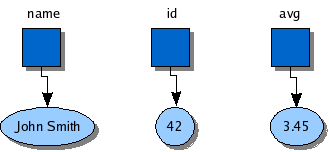
\includegraphics[scale=0.7]{variables.png}
\end{center}
\end{frame}
    
\begin{frame}[fragile]
\frametitle{Dodela vrednosti}
\begin{itemize}
  \item kada se nova referenca dodeli promenljivoj, stara referenca se gubi
\end{itemize}
\begin{minted}[linenos=false,fontsize=\small]{python}
id = 70
\end{minted}
\begin{center}
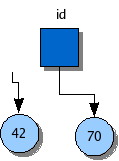
\includegraphics[scale=0.7]{newref.png}
\end{center}
\end{frame}
  
\begin{frame}[fragile]
\frametitle{Dodela vrednosti}
\begin{itemize}
  \item nova referenca može biti na objekat drugog tipa
\end{itemize}
\begin{minted}[linenos=false,fontsize=\small]{python}
id = "smith"
\end{minted}
\begin{center}
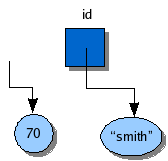
\includegraphics[scale=0.7]{diffref.png}
\end{center}
\end{frame}
  
\begin{frame}[fragile]
\frametitle{Konstante: ne postoje}
\begin{itemize}
  \item dve konstante u Javi
\end{itemize}
\begin{minted}[linenos=false,fontsize=\small]{java}
final double TAX_RATE = 0.06;
final int MAX_SIZE = 100;
\end{minted}
\begin{itemize}
  \item konvencija za promenljive kojima nećemo menjati vrednost: uppercase
\end{itemize}
\begin{minted}[linenos=false,fontsize=\small]{python}
TAX_RATE = 0.06
MAX_SIZE = 100
\end{minted}
\end{frame}

\begin{frame}[fragile]
\frametitle{Aritmetički operatori}
\begin{tabular}{lp{5cm}}
  \textbf{operator} & \textbf{napomena} \\ \hline
  \texttt{+} & sabiranje \\ \hline
  \texttt{-} & oduzimanje \\ \hline
  \texttt{*} & množenje \\ \hline
  \texttt{/} & deljenje \\ \hline
  \texttt{**} & stepenovanje \\ \hline
  \texttt{//} & celobrojno deljenje \\ \hline
  \texttt{\%} & ostatak
\end{tabular}
\begin{itemize}
  \item ima \texttt{+=}, \texttt{-=}, \dots
  \item nema \texttt{++} i \texttt{--}
\end{itemize}
\end{frame}
    
\begin{frame}[fragile]
\frametitle{Mešanje numeričkih tipova: \texttt{1 + 2.0}}
\begin{itemize}
  \item operand manjeg ranga se konvertuje u veći rang
  \item rang tipova: \\
    \texttt{complex} > \texttt{float} > \texttt{int}
\end{itemize}
\end{frame}
    
\begin{frame}[fragile]
\frametitle{Konverzija tipova}
\begin{itemize}
  \item automatska konverzija samo za numeričke tipove unutar numeričkih izraza
  \item sve ostale konverzije moraju biti eksplicitne
\end{itemize}
\begin{minted}[linenos=false,fontsize=\small]{python}
x = 100
y = "abc"
z = y + str(x)
\end{minted}
\end{frame}

\begin{frame}[fragile]
\frametitle{Glavni program i Java}
\begin{minted}[linenos=false,fontsize=\small]{java}
// Sumation.java
// Compute the sum of the first 100 integer values and print
// the results.
public class Summation {
  public static void main(String[] args) {
    final int NUM_VALUES = 100;
    int summation = 0;
    int i = 0;

    while (i <= NUM_VALUES) {
      summation = summation + 1;
      i = i + 1;
    }

    System.out.println("The sum of the first " + NUM_VALUES
                        + " integers is " +  summation);
  }
}
\end{minted}
\end{frame}
  
\begin{frame}[fragile]
\frametitle{Glavni program i Python}
\begin{minted}[linenos=false,fontsize=\small]{python}
# summation.py
# Compute the sum of the first 100 integer values and print
# the results.

# Initialize a constant variable.
NUM_VALUES = 100

# Compute the sum.
summation = 0
i = 1
while i <= NUM_VALUES:
   summation = summation + i
   i = i + 1

# Print the results.
print("The sum of the first", NUM_VALUES,
      "integers is", summation)
\end{minted}
\end{frame}
  
\section{Funkcije}

\begin{frame}[fragile]
\frametitle{Funkcija}
\begin{itemize}
  \item slična \texttt{static} metodi u Javi
  \item koriste se nezavisno od objekata
  \item u Pajtonu se ne definišu unutar klase
  \item (ali i mogu)
\end{itemize}
\begin{minted}[linenos=false,fontsize=\small]{python}
x = 100
y = "abc"
z = y + str(x)
\end{minted}
\end{frame}
  
\begin{frame}[fragile]
\frametitle{Ugrađene funkcije}
\begin{itemize}
  \item neke funkcije su deo jezika kao ugrađene (built-in)
  \item uvek su dostupne
\end{itemize}
\begin{minted}[linenos=false,fontsize=\small]{python}
# Compute the absolute value of the integer x
y = abs(x)
\end{minted}
\end{frame}
  

\end{document}